% Template for a Computer Science Tripos Part II project dissertation
\documentclass[12pt,a4paper,twoside,openright]{report}
\usepackage[pdfborder={0 0 0}]{hyperref}    % turns references into hyperlinks
\usepackage[margin=25mm]{geometry}  % adjusts page layout
\usepackage{graphicx}  % allows inclusion of PDF, PNG and JPG images
\usepackage{verbatim}
\usepackage{docmute}   % only needed to allow inclusion of proposal.tex

\raggedbottom                           % try to avoid widows and orphans
\sloppy
\clubpenalty1000%
\widowpenalty1000%

\renewcommand{\baselinestretch}{1.1}    % adjust line spacing to make
                                        % more readable

\begin{document}

\bibliographystyle{plain}


%%%%%%%%%%%%%%%%%%%%%%%%%%%%%%%%%%%%%%%%%%%%%%%%%%%%%%%%%%%%%%%%%%%%%%%%
% Title


\pagestyle{empty}

\rightline{\LARGE \textbf{Martin Richards}}

\vspace*{60mm}
\begin{center}
\Huge
\textbf{How to write a dissertation in \LaTeX} \\[5mm]
Computer Science Tripos -- Part II \\[5mm]
St John's College \\[5mm]
\today  % today's date
\end{center}

%%%%%%%%%%%%%%%%%%%%%%%%%%%%%%%%%%%%%%%%%%%%%%%%%%%%%%%%%%%%%%%%%%%%%%%%%%%%%%
% Proforma, table of contents and list of figures

\pagestyle{plain}

\chapter*{Proforma}

{\large
\begin{tabular}{ll}
Name:               & \bf Martin Richards                       \\
College:            & \bf St John's College                     \\
Project Title:      & \bf How to write a dissertation in \LaTeX \\
Examination:        & \bf Computer Science Tripos -- Part II, July 2001  \\
Word Count:         & \bf 1587\footnotemark[1]
                      (well less than the 12000 limit)  \\
Project Originator: & Dr M.~Richards                    \\
Supervisor:         & Dr Markus Kuhn                    \\ 
\end{tabular}
}
\footnotetext[1]{This word count was computed
by \texttt{detex diss.tex | tr -cd '0-9A-Za-z $\tt\backslash$n' | wc -w}
}
\stepcounter{footnote}


\section*{Original Aims of the Project}

To write a demonstration dissertation\footnote{A normal footnote without the
complication of being in a table.} using \LaTeX\ to save
student's time when writing their own dissertations. The dissertation
should illustrate how to use the more common \LaTeX\ constructs. It
should include pictures and diagrams to show how these can be
incorporated into the dissertation.  It should contain the entire
\LaTeX\ source of the dissertation and the makefile.  It should
explain how to construct an MSDOS disk of the dissertation in
Postscript format that can be used by the book shop for printing, and,
finally, it should have the prescribed layout and format of a diploma
dissertation.


\section*{Work Completed}

All that has been completed appears in this dissertation.

\section*{Special Difficulties}

Learning how to incorporate encapulated postscript into a \LaTeX\
document on both Ubuntu Linux and OS X.
 
\newpage
\section*{Declaration}

I, [Name] of [College], being a candidate for Part II of the Computer
Science Tripos [or the Diploma in Computer Science], hereby declare
that this dissertation and the work described in it are my own work,
unaided except as may be specified below, and that the dissertation
does not contain material that has already been used to any substantial
extent for a comparable purpose.

\bigskip
\leftline{Signed [signature]}

\medskip
\leftline{Date [date]}

\tableofcontents

\listoffigures

\newpage
\section*{Acknowledgements}

This document owes much to an earlier version written by Simon Moore
\cite{Moore95}.  His help, encouragement and advice was greatly 
appreciated.

%%%%%%%%%%%%%%%%%%%%%%%%%%%%%%%%%%%%%%%%%%%%%%%%%%%%%%%%%%%%%%%%%%%%%%%
% now for the chapters

\pagestyle{headings}

\chapter{Introduction}

\section{Overview of the files}

This document consists of the following files:

\begin{itemize}
\item \texttt{makefile} --- The makefile for the dissertation and
                         Project Proposal
\item \texttt{diss.tex} --- The dissertation
\item \texttt{proposal.tex}  --- The project proposal 
\item \texttt{figs} -- A directory containing diagrams and pictures
\item \texttt{refs.bib} --- The bibliography database
\end{itemize}

\section{Building the document}

This document was produced using \LaTeXe which is based upon
\LaTeX\cite{Lamport86}.  To build the document you first need to
generate \texttt{diss.aux} which, amongst other things, contains the
references used.  This if done by executing the command:

\texttt{pdflatex diss}

\noindent
Then the bibliography can be generated from \texttt{refs.bib} using:

\texttt{bibtex diss}

\noindent
Finally, to ensure all the page numbering is correct run \texttt{pdflatex}
on \texttt{diss.tex} until the \texttt{.aux} files do not change.  This
usually takes 2 more runs.

\subsection{The makefile}

To simplify the calls to \texttt{pdflatex} and \texttt{bibtex}, 
a makefile has been provided, see Appendix~\ref{makefile}. 
It provides the following facilities:

\begin{description}

\item\texttt{make} \\
 Display help information.

\item\texttt{make proposal.pdf} \\
 Format the proposal document as a PDF.

\item\texttt{make view-proposal} \\
 Run \texttt{make proposal.pdf} and then display it with a Linux PDF viewer
 (preferably ``okular'', if that is not available fall back to ``evince'').

\item\texttt{make diss.pdf} \\
 Format the dissertation document as a PDF.

\item\texttt{make count} \\
Display an estimate of the word count.

\item\texttt{make all} \\
Construct \texttt{proposal.pdf} and \texttt{diss.pdf}.

\item\texttt{make pub} \\ Make \texttt{diss.pdf}
and place it in my \texttt{public\_html} directory.

\item\texttt{make clean} \\ Delete all intermediate files except the
source files and the resulting PDFs. All these deleted files can
be reconstructed by typing \texttt{make all}.

\end{description}


\section{Counting words}

An approximate word count of the body of the dissertation may be
obtained using:

\texttt{wc diss.tex}

\noindent
Alternatively, try something like:

\verb/detex diss.tex | tr -cd '0-9A-Z a-z\n' | wc -w/


\chapter{Preparation}

This chapter is empty!


\chapter{Implementation}

\section{Verbatim text}

Verbatim text can be included using \verb|\begin{verbatim}| and
\verb|\end{verbatim}|. I normally use a slightly smaller font and
often squeeze the lines a little closer together, as in:

{\renewcommand{\baselinestretch}{0.8}\small
\begin{verbatim}
GET "libhdr"
 
GLOBAL { count:200; all  }
 
LET try(ld, row, rd) BE TEST row=all
                        THEN count := count + 1
                        ELSE { LET poss = all & ~(ld | row | rd)
                               UNTIL poss=0 DO
                               { LET p = poss & -poss
                                 poss := poss - p
                                 try(ld+p << 1, row+p, rd+p >> 1)
                               }
                             }
LET start() = VALOF
{ all := 1
  FOR i = 1 TO 12 DO
  { count := 0
    try(0, 0, 0)
    writef("Number of solutions to %i2-queens is %i5*n", i, count)
    all := 2*all + 1
  }
  RESULTIS 0
}
\end{verbatim}
}

\section{Tables}

\begin{samepage}
Here is a simple example\footnote{A footnote} of a table.

\begin{center}
\begin{tabular}{l|c|r}
Left      & Centred & Right \\
Justified &         & Justified \\[3mm]
%\hline\\%[-2mm]
First     & A       & XXX \\
Second    & AA      & XX  \\
Last      & AAA     & X   \\
\end{tabular}
\end{center}

\noindent
There is another example table in the proforma.
\end{samepage}

\section{Simple diagrams}

Simple diagrams can be written directly in \LaTeX.  For example, see
figure~\ref{latexpic1} on page~\pageref{latexpic1} and see
figure~\ref{latexpic2} on page~\pageref{latexpic2}.

\begin{figure}
\setlength{\unitlength}{1mm}
\begin{center}
\begin{picture}(125,100)
\put(0,80){\framebox(50,10){AAA}}
\put(0,60){\framebox(50,10){BBB}}
\put(0,40){\framebox(50,10){CCC}}
\put(0,20){\framebox(50,10){DDD}}
\put(0,00){\framebox(50,10){EEE}}

\put(75,80){\framebox(50,10){XXX}}
\put(75,60){\framebox(50,10){YYY}}
\put(75,40){\framebox(50,10){ZZZ}}

\put(25,80){\vector(0,-1){10}}
\put(25,60){\vector(0,-1){10}}
\put(25,50){\vector(0,1){10}}
\put(25,40){\vector(0,-1){10}}
\put(25,20){\vector(0,-1){10}}

\put(100,80){\vector(0,-1){10}}
\put(100,70){\vector(0,1){10}}
\put(100,60){\vector(0,-1){10}}
\put(100,50){\vector(0,1){10}}

\put(50,65){\vector(1,0){25}}
\put(75,65){\vector(-1,0){25}}
\end{picture}
\end{center}
\caption{A picture composed of boxes and vectors.}
\label{latexpic1}
\end{figure}

\begin{figure}
\setlength{\unitlength}{1mm}
\begin{center}

\begin{picture}(100,70)
\put(47,65){\circle{10}}
\put(45,64){abc}

\put(37,45){\circle{10}}
\put(37,51){\line(1,1){7}}
\put(35,44){def}

\put(57,25){\circle{10}}
\put(57,31){\line(-1,3){9}}
\put(57,31){\line(-3,2){15}}
\put(55,24){ghi}

\put(32,0){\framebox(10,10){A}}
\put(52,0){\framebox(10,10){B}}
\put(37,12){\line(0,1){26}}
\put(37,12){\line(2,1){15}}
\put(57,12){\line(0,2){6}}
\end{picture}

\end{center}
\caption{A diagram composed of circles, lines and boxes.}
\label{latexpic2}
\end{figure}



\section{Adding more complicated graphics}

The use of \LaTeX\ format can be tedious and it is often better to use
encapsulated postscript (EPS) or PDF to represent complicated graphics.
Figure~\ref{epsfig} and~\ref{xfig} on page \pageref{xfig} are
examples. The second figure was drawn using \texttt{xfig} and exported in
{\tt.eps} format. This is my recommended way of drawing all diagrams.


\begin{figure}[tbh]
\centerline{
\includegraphics{figs/cuarms.pdf}}
\caption{Example figure using encapsulated postscript}
\label{epsfig}
\end{figure}

\begin{figure}[tbh]
\vspace{4in}
\caption{Example figure where a picture can be pasted in}
\label{pastedfig}
\end{figure}


\begin{figure}[tbh]
\centerline{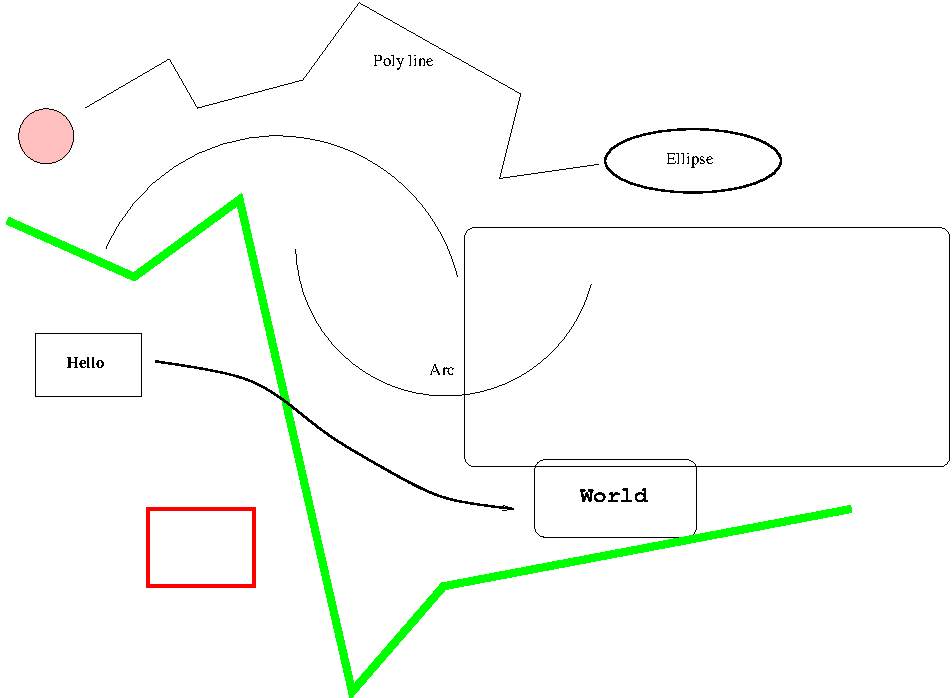
\includegraphics{figs/diagram.pdf}}
\caption{Example diagram drawn using \texttt{xfig}}
\label{xfig}
\end{figure}


\chapter{Evaluation}

\section{Printing and binding}

Use a ``duplex'' laser printer that can print on both sides to print
two copies of your dissertation. Then bind them, for example using the
comb binder in the Computer Laboratory Library.

\section{Further information}

See the Unix Tools notes at

\url{http://www.cl.cam.ac.uk/teaching/current-1/UnixTools/materials.html}


\chapter{Conclusion}

I hope that this rough guide to writing a dissertation is \LaTeX\ has
been helpful and saved you time.


%%%%%%%%%%%%%%%%%%%%%%%%%%%%%%%%%%%%%%%%%%%%%%%%%%%%%%%%%%%%%%%%%%%%%
% the bibliography
\addcontentsline{toc}{chapter}{Bibliography}
\bibliography{refs}

%%%%%%%%%%%%%%%%%%%%%%%%%%%%%%%%%%%%%%%%%%%%%%%%%%%%%%%%%%%%%%%%%%%%%
% the appendices
\appendix

\chapter{Latex source}

\section{diss.tex}
{\scriptsize\verbatiminput{diss.tex}}

\section{proposal.tex}
{\scriptsize\verbatiminput{proposal.tex}}

\chapter{Makefile}

\section{makefile}\label{makefile}
{\scriptsize\verbatiminput{makefile.txt}}

\section{refs.bib}
{\scriptsize\verbatiminput{refs.bib}}


\chapter{Project Proposal}

\documentclass[11pt]{article}
\usepackage{a4wide,parskip,times}
\usepackage{color}
\usepackage{tabulary}

\usepackage[
backend=biber,
sorting=ynt
]{biblatex}
\addbibresource{main.bib}

\begin{document}

\begin{abstract}


There has recently been an increasing need for fast analysis of 
graph-structured data, which has led to the development of several graph-centric
alternatives to traditional relational databases. Although these ensure the
fast execution of queries which fit within this graph-centric model,
inevitably a compromise has been made, and other queries perform less
efficiently than they would have done with a relational database. I propose
the development of a query language enabling intelligent dispatch of optimised
queries either directly to a relational database, or through a graph-centric query processing
layer.

\end{abstract}

\section{Introduction, approach and outcomes}

Graph databases are an alternative to traditional relational databases, which
improve access speeds for some queries by prioritising access to related
entities, rather than expecting traversal through a fixed schema. This can
provide huge performance improvements for graph-centric queries, such as
shortest path queries. For other queries, however -- such as aggregation of
otherwise unrelated data items -- it is far more efficient to rely on a fixed
schema for fast access. A recent project\cite{crackle} has shown that it is
possible to unify both graph and relational database paradigms by providing
graph-focused pre-fetching of data from an underlying relational database.  I
now aim to further unify the systems in two ways.

My first contribution is to present a declarative query language 
targeting this hybrid system. Two interfaces to the data exist: going
straight to the relational database, or through the graph-centric query
layer. The language will be amenable to analysis, to
allow an interpreter to determine which queries will be 
handled more effectively by which interface, and to efficiently 
dispatch these targeted queries.

My second contribution is to extend the performance benefits
by decomposing
user queries and extracting opportunities for parallelisation
Decades of research have worked on
optimising SQL queries in this way, and some ideas from the domain of relational
query planning will provide insights into increasing the performance of graph
queries.

Another challenge of the work is ensuring usability of the query language. Queries targeting a graph database queries are a very different
to those for relational databases, as they are used to solve different sorts of problems. I will pay careful attention that both paradigms are sufficiently
expressible, and that the resulting language is coherent.

To evaluate my project, firstly, it will be important to show that the system provides a performance improvement
over current solutions. I will make comparisons against Neo4J\cite{neo4j} and PostgreSQL\cite{postgres}. I expect the two systems to run slightly faster on queries for which they are specialised, but that my system will significantly outperform them on queries for which they are not particularly optimised. I will also present an independent performance evaluation of my optimisations,
exploring their impact and limitations. Finally, I will evaluate the usability of the resulting
language to ensure that the platform is sufficiently expressive
without being incoherent.

% What about discussion of read-only accesses vs updates too?

If time allows, there are a few possible directions for extension. Firstly, 
the nature of the query layer places no restriction on
the type of the underlying data store. It would be interesting to explore the
effect of using other data sources in place of a relational database.
There may also be opportunities here for
query optimisation which are not present when using PostgreSQL. Finally, 
the discussion above has considered only the efficient retrieval of data.
Clearly it would also be desirable to allow updates, though this introduces
complexity with regards to the consistency of prefetched data. It would be
instructive to start work in this direction in order to have some idea of
the particular difficulties which would need overcoming.

\section{Work Plan}

The structure of my research will follow three main stages. Firstly, I will
work on the dispatch mechanism for user queries. I intend to identify optimal
dispatch strategies by taking a ``problem-first'' approach, and looking for
patterns in the differences between the kinds of problems which tend to
currently be approached using graph databases, and those which use relational
databases. I expect this work to roughly continue until the start of Lent
term.

During the course of Lent term, I will consider the problem of query
optimisation. I will proceed by performing tests to identify a few possible
avenues for performance improvements, before implementing the most promising
ones and measuring their effects. The design of the query language itself will
be ongoing throughout the entirety of the project, to ensure both that the
information retrieval problem space is adequately covered, and that
opportunities for optimisation are adequately exposed.

Finally, I will use the remaining time available to perform more detailed
evaluation, refine the usability of the language, and prepare the write up.

A detailed work plan is included overleaf. In this plan, bold items represent fairly
objective milestones, which should help ensure that I do not fall behind.


\begin{center}
\begin{tabulary}{\linewidth}{|CLLL|}
\hline
 Week & Date & Work to complete & \\
 \hline
 1  & 16th November--29th November & Background reading and prepare \textbf{revised proposal}. & \\[3ex]
 3  & 30th November--13th December & Set up development environment and \textbf{replicate Crackle results}. & \\[3ex]
 5  & 14th December--27th December & Expand Crackle results (different data/different queries). & \\[3ex]
 7  & 28th December--10th January & Collect results and \textbf{establish preliminary dispatch strategy}.  & \\[3ex]
 9  & 11th January--24th January & Read around area of query planning and optimisation. & \\[3ex]
 11 & 25th January--7th February & Perform tests to identify \textbf{two or three possible avenues for optimisation}. & \\[3ex]
 13 & 8th February--21st February & Implement first optimisations. & \\[3ex]
 15 & 22nd February--6th March & \textbf{Finish implementing optimisations} and \textbf{prepare progress report}.&\\[3ex]
 17 & 7th March--20th March & \textbf{Finish design of DSL}. & \\[3ex]
 19 & 21st March--3rd April & Conduct thorough performance evaluations. & \\[3ex]
 21 & 4th April--17th April & Evaluate DSL and begin write-up. & \\[3ex]
 23 & 18th April--1st May & Continue write-up. Complete an \textbf{initial draft of 11-13,500 words}.  & \\[3ex]
 25 & 2nd May--15th May & Refine draft and correct word count. & \\[3ex]
 27 & 16th May--29th May & Final edits and \textbf{submission}. & \\[3ex]
 (29)&30th May--6th June & Prepare \textbf{presentation}. & \\[3ex]
 \hline
\end{tabulary}
\end{center}

\end{document}


\end{document}
